% Basic stuff
\documentclass[a4paper,10pt]{article}
\usepackage[nswissgerman]{babel}
\usepackage[utf8]{inputenc}
\usepackage[T1]{fontenc}

% 3 column landscape layout with fewer margins
\usepackage[landscape, left=0.75cm, top=1cm, right=0.75cm, bottom=1.5cm, footskip=15pt]{geometry}
\usepackage{flowfram}
\ffvadjustfalse
\setlength{\columnsep}{1cm}
\Ncolumn{3}

% define nice looking boxes
\usepackage[many]{tcolorbox}

% a base set, that is then customised
\tcbset {
  base/.style={
    boxrule=0mm,
    leftrule=1mm,
    left=1.75mm,
    arc=0mm, 
    fonttitle=\bfseries, 
    colbacktitle=black!10!white, 
    coltitle=black, 
    toptitle=0.75mm, 
    bottomtitle=0.25mm,
    title={#1}
  }
}

\usepackage[T1]{fontenc}
\usepackage[nswissgerman]{babel}
\usepackage{gensymb}
\usepackage{multicol}
\usepackage{float}
\usepackage{pgfplots}
\pgfplotsset{compat=newest}
\usepackage{changepage}

\usepackage{zref-totpages}
\makeatletter
\renewcommand{\@evenfoot}{\hfil \thepage{}/\ztotpages\hfil}
\renewcommand{\@oddfoot}{\@evenfoot}
\makeatother


% define nice looking boxes
\usepackage[many]{tcolorbox}

% a base set, that is then customised

\tcbset {
  base/.style={
    boxrule=0mm,
    leftrule=0mm,
    left=1.75mm,
    arc=1mm, 
    fonttitle=\bfseries, 
    colbacktitle=black!10!white, 
    coltitle=black, 
    toptitle=0.75mm, 
    bottomtitle=0.25mm,
    title={#1}
  }
}

\definecolor{bluetitle}{RGB}{210, 235, 255}
\definecolor{blueframe}{RGB}{146, 208, 255}
\definecolor{blueback}{RGB}{236, 247, 255}
\newtcolorbox{mainbox}[1]{
  colframe=blueframe, 
  base={#1},
  colbacktitle=bluetitle,
  colback=blueback,
}

\newtcolorbox{subbox}[1]{
  colframe=black!20!white,
  base={#1}
}


% Mathematical typesetting & symbols
\usepackage{amsthm, mathtools, amssymb} 
\usepackage{marvosym, wasysym}
%\usepackage{derivative}
\newcommand{\pdv}[2]{\frac{\partial #1}{\partial #2}}



% Tables
\usepackage{tabularx, multirow}
\usepackage{booktabs}

% Make enumerations more compact
\usepackage{enumitem}
\setitemize{itemsep=0.5pt}
\setenumerate{itemsep=0.75pt}

% To include sketches & PDFs
\usepackage{graphicx}

% For hyperlinks
\usepackage{hyperref}
\hypersetup{
  colorlinks=true
}

% Metadata
\title{Analysis II}
\author{by Silvan Metzker}
\date{January 2024}

% Math helper stuff
\def\limn{\lim_{n\to \infty}}
\def\limxo{\lim_{x\to 0}}
\def\limxi{\lim_{x\to\infty}}
\def\limxn{\lim_{x\to-\infty}}
\def\sumk{\sum_{k=1}^\infty}
\def\sumn{\sum_{n=0}^\infty}
\def\R{\mathbb{R}}
\def\C{\mathbb{C}}
\def\Q{\mathbb{Q}}
\def\N{\mathbb{N}}
\def\X{\mathcal{X}}
\def\dx{\text{ d}x}

\begin{document}

\setlength{\abovedisplayskip}{3pt}
\setlength{\belowdisplayskip}{3pt}
\setlength{\abovedisplayshortskip}{3pt}
\setlength{\belowdisplayshortskip}{3pt}

\begin{center}
	\vspace{1cm}
	{\Large \textsc{Cheat Sheet}\par}
	{\huge\bfseries Analysis II\par}
	\vspace{0.5cm}
	{\Large\itshape Silvan Metzker\par}
	{\large Januar 2024\par}
	\vspace{0.4cm}
	{\textbf{Lizenz:} CC BY-SA 4.0}
\end{center}

\section{Differentialgleichungen}
\begin{mainbox}{Definition lineare DGL}
	Eine gewöhnliche lineare Differentialgleichung ist eine Gleichung, welche Ableitungen enthält. Sie hat die Form $$y^{(n)} + a_{n-1} y^{(n-1)} + \cdots + a_0y = b(x)$$
	wo die Koeffizienten $a_0, \ldots, a_{n-1}$ komplexe Funktionen auf $I \subset \R$ sind, welche von $x$ abhängig sein können. Wenn $b(x) = 0$ gilt, ist die DGL (zugehörig) homogen, ansonsten inhomogen. 
\end{mainbox}
Die Menge $S$ an Lösungen ist ein Subset des Raums der komplexen Funktionen auf $I$ mit Dimension $n$. \\
$S_0$ das Set der Lösungen zu einer homogenen DGL. Für ein $b(x)$ ist die Menge der Lösungen 
$$S_b = \{f_h + f_p \mid f_h \in S_0\}.$$
\subsubsection*{Lineare DGL erkennen}
\begin{itemize}
	\item keine Koeffizienten vor der höchsten Ableitung
	\item alle Koeffizienten sind stetige Funktionen
	\item keine Produkte von $y$ oder deren Ableitungen
	\item keine Potenzen von $y$ oder deren Ableitungen
	\item keine Funktionen von $y$ oder deren Ableitungen
\end{itemize}


\subsection{Lineare DGL erster Ordnung}
Wir betrachten DGL der Form $$y' + a(x)y = b(x)$$
\begin{enumerate}[label=\textbf{\arabic*.}]
	\item \textbf{Homogene Lösung:} Löse nach $y$.
	      \begin{align*}
	      	y' + a(x)y   & = 0                                             \\
	      	\frac{y'}{y} & = -a(x)                                         \\
	      	\ln(y)       & = -A(x)+C                                       \\
	      	f_0 := y     & = e^{-A(x)+C} = z \cdot e^{-A(x)}\quad z \in \C 
	      \end{align*}
	\item \textbf{Partikuläre Lösung:} Verwende entweder ``Variation der Konstanten'' oder ``Fundiertes Raten''.
	\item \textbf{Allgemeine Lösung:} Vereinige beide Lösungen,
	      $f_{0}+ \sum\limits_{j=1}^{n}\alpha_{j}f_{j}$ mit $\alpha_{j} \in \mathbb{C}$
	\item \textbf{Anfangswerte:} Einsetzen der Anfangswerte in die allg. Lösung $\rightarrow$ LGS für $\alpha_{1},\dots,\alpha_{k}$ mit eindeutiger Lösung.
	        
\end{enumerate}
\subsection{Variation der Konstanten}
Sei $f_p = z(x)e^{-A(x)}$ für eine Funktion $z: I \to \C$. Dann ist $z'(x) = b(x) e^{A(x)}$ und somit $$z(x) = \int_{x_0}^x b(t) e^{A(t)} \mathop{dt}$$ Daraus erhalten wir $$f_p = \int_{x_0}^x b(t) e^{A(t)} \mathop{dt} \cdot e^{-A(t)}$$


\subsection{Separation der Variabeln}
DGL der Form $y'=\frac{1}{a(y)}\cdot b(x)$ mit $a,b$ stetig, $a(y)\neq 0$.  
\begin{align*}
	&\Longleftrightarrow a(y)\cdot y' = b(x)\\
	&\Longleftrightarrow \int a(y)\cdot y'(x)\ dx = \int b(x)\ dx + c\\
	&\Longleftrightarrow A(y) = B(x)+c \quad(\text{mit }A,B\text{ als Stammfunkt.})\\
	&\Longleftrightarrow y = A^{-1}(B(x)+c)
\end{align*}

\subsection{Fundiertes Raten}

Wenn $b(x)$ von einer bestimmten Form ist, versuchen wir folgende $f_p$, wobei wir unseren Versuch in die DGL einsetzen, was uns dann ein Gleichungssystem für die Konstanten gibt:




\begin{center}
	\renewcommand*{\arraystretch}{1.6}
	\begin{tabular}{cc} 
		\toprule
		$b(x)$                                & Raten                                                               \\ 
		\midrule     
		$P_n(x)$                              & $R_{n+k}(x)$                                                        \\
		$a \cdot e^{\alpha x}$                & $b \cdot e^{\alpha x}$                                              \\
		$a^\star \sin(\beta x)+b^\star \cos(\beta x)$ & $c \sin(\beta x) + d \cos(\beta x)$                                 \\
		$a e^{\alpha x} \sin(\beta x)$        & $e^{\alpha x} \Big( c \sin(\beta x) + d \cos(\beta x) \Big)$        \\
		$b e^{\alpha x} \cos(\beta x)$        & $e^{\alpha x} \Big( c \sin(\beta x) + d \cos(\beta x) \Big)$        \\
		$P_n e^{\alpha x}$                    & $R_n \cdot e^{\alpha x}$                                            \\
		$P_n e^{\alpha x} \sin(\beta x)$      & $e^{\alpha x} \left( R_n \sin(\beta x) + S_n \cos(\beta x) \right)$ \\
		$P_n e^{\alpha x} \cos(\beta x)$      & $e^{\alpha x} \left( R_n \sin(\beta x) + S_n \cos(\beta x) \right)$ \\
		\bottomrule
	\end{tabular}
\end{center}

\noindent $P_n, R_n $ und $S_n$ sind Polynome abh. von $x$ und $k$ ist die Ordnung der kleinsten Ableitung im homogenen Teil. \\
Gilt auch für $a^\star=0$ oder $b^\star=0$.

\begin{enumerate}
	\item Wenn $b(x)$ eine Linearkombination der Basisfunktionen ist, dann versuche eine Linearkombination.
	\item Wenn die geratene Lösung der homogenen Lösung entspricht, dann multipliziere mit $x^m$, wobei $x$ die Vielfachheit der Wurzel ist.
\end{enumerate}

\subsection{Lineare DGL mit konstanten Koeff.}
Wir wollen lösen: $y^{(k)}+a_{k-1}y^{(k-1)}+\dots + a_{0}y=b$.\\
Dann bekommt man das \textit{Charakteristische Polynom}:  
$$\iff \lambda^{k}+a_{k-1}\lambda^{(k-1)}+\dots + a_{0}=0$$
Dann ist die homogene Lösung eine Linearkombination aus $f_\ell =x^{j}e^{\lambda_{i}x}$ für jede Nullstelle $\lambda_i$ und dessen Vielfachheit $m$, also $j\in \{ 0,...,m-1 \}$.\\
Falls Reelle Lösungen gesucht und $a_i \in \mathbb{R}$ und seien $\lambda_{i,i+1} =\beta \pm \gamma i$ zwei Nullstellen des charakteristischen Polynom. \\Dann gilt $f_{i}=e^{\beta x}\cos (\gamma x)$ und $f_{i+1}=e^{\beta x}\sin (\gamma x)$.\\

Um eine partikuläre Lösung zu finden, können wir wieder fundiertes Raten oder Variation der Konstanten verwenden. 
Variation der Konstanten funktioniert wie folgt (hier 2D, bzw. $\ell\in \{1,2\}$):

\begin{enumerate}[label=(\arabic*)]
	\item Nimm an, dass die homogene Lösung \\
	$f_h = z_1 f_1 + z_2 f_2$ ist, für $z_1, z_2 \in \mathbb C$.
	\item Versuche nun $f_p = z_1(x) f_1 + z_2(x) f_2$
	\item Löse das folgende System
	      \begin{align*}
	      	z_1'(x) f_1 + z_2'(x) f_2   & = 0    \\
	      	z_1'(x) f_1' + z_2'(x) f_2' & = b(x) \\
	      \end{align*}
	      Hier gehen wir wie folgt vor:
	      \begin{align*}
	      	W                & = f_1 f_2' - f_2 f_1' \neq 0                                 \\
	      	\Rightarrow z_1' & = \frac{-f_2 b}{W} \; , z_2' = \frac{-f_1 b}{W}              \\
	      	\Rightarrow f_p  & = -f_1 \int \frac{f_2 b}{W} dt + f_2 \int \frac{f_1 b}{W} dt 
	      \end{align*}
\end{enumerate}

\section{Ableitungen in \texorpdfstring{$\R^n$}{Rⁿ}}
\begin{subbox}{Monom}
	Ein Monom vom Grad $e$ ist
	\begin{align*}
		(x_1, \ldots, x_n) \mapsto x_1^{d_1}\cdot \ldots \cdot x_n^{d_n} \\
		e = d_1 + \ldots + d_n                                           
	\end{align*}
	$\to$ ein Polynom, das nur aus einem Glied besteht.
\end{subbox}
\begin{mainbox}{Polynom}
	Ein Polynom mit $n$ Variablen vom Grad $d$ ist eine endliche Summe von Monomen mit Grad $e \le d$.
\end{mainbox}

\subsection{Konvergenz}
\begin{enumerate}
	\item Skalarprodukt: $\left< x,y\right> = \sum_{i=0} x_i \cdot y_i$
	\item Euklidische Norm: $||x|| := \sqrt{x_2^1 + \cdots + x_n^2}$ mit den folgenden Eigenschaften:
	      \begin{enumerate}
	      	\item $||x|| \ge 0, ||x|| = 0 \iff x = 0$
	      	\item $||\lambda x|| = |\lambda| \cdot ||x||, \forall \lambda \in \R$
	      	\item $||x+y|| \le ||x|| + ||y||$
	      	\item $|\left<x,y\right>| \le ||x|| \cdot ||y||$
	      \end{enumerate}
\end{enumerate}

\begin{mainbox}{Definition Konvergenz}
	Sei $(x_k)_{k \in \mathbb{N}},\ x_k \in \R^n$. Die folgenden Definitionen sind für $\lim_{k\to\infty}x_k = y$ äquivalent:
	\begin{enumerate}
		\item $\forall \varepsilon > 0,\ \exists N \ge 1$ so dass $\forall k \ge N \ ||x_k - y|| < \varepsilon$.
		\item Für jedes $i \in \{1,2,\dots, n\}$ konvergiert die Folge $(x_{k,i})_k$ von reellen Zahlen nach $y_i$.
		\item Die Folge der reellen Zahlen $||x_k - y||$ konvergiert nach $0$.
	\end{enumerate}
\end{mainbox}
\subsection{Stetigkeit}
Sei $f: \X \subset \R^n \to \R^m$  und $x_0 \in \X$. \\
Funktion $f$ ist \textbf{stetig in $\bf x_0$}, falls eine der folgenden Bedingungen erfüllt ist:
\begin{enumerate}
	\item $\forall \varepsilon > 0,\ \exists \delta > 0$ so dass $x \in \X,\ ||x - x_0|| < \delta \implies ||f(x) - f(x_0)|| < \varepsilon$.
	\item Für alle Folgen $(x_k)$ in $X$ mit $\lim x_k = x_0$ gilt $\lim f(x_k) = f(\lim x_k)$.
	\item $\displaystyle\lim_{\substack{x \to \infty \\ x \neq x_{0}}}f(x)=f(x_{0}) $
\end{enumerate}
Funktion $f$ ist \textbf{stetig in $\bf \X$} falls $f$ für jeden Punkt $x_0 \in \X$ stetig ist. Es gilt:
\begin{enumerate}
	\item $f(x = x_1, \ldots, x_n) \mapsto (f_1(x),\ldots,f_m(x))$ und $f_i: \R^n \to \R$. Dann gilt: \\
	$f$ stetig $\iff \forall i = 1, \ldots, m \ f_i$ stetig.
	\item Polynome sind stetig.
	\item Summen + Produkte von stetigen Funktionen sind stetig.
	\item Funktionen unterschiedlicher Variablen sind stetig, falls alle Variablen stetig sind.
	\item Verknüpfungen stetiger Funktionen sind stetig.
\end{enumerate}


\begin{mainbox}{Sandwich-Lemma}
	Wenn $f, g, h: \R^n \to \R$ Funktionen für die gilt, dass $\forall x \in \R^n,\ f(x) < g(x) < h(x)$, dann gilt
	$$\lim_{x\to a} f(x) = \lim_{x \to a} h(x) = L \implies \lim_{x\to a} g(x) = L$$
\end{mainbox}

\begin{mainbox}{Definition Limit zu $x_0$}
Sei $X \subseteq \mathbb{R}^{n}$ und $f:X\to R^{m}$. Sei $x_{0}\in X$ und $y\in\mathbb{R}^{m}$. Falls:
\begin{gather*}
\forall \varepsilon>0,\ \exists \delta>0,\ \forall x \in X,\ x\neq x_{0},\ \\
\|x-x_{0}\|<\delta\implies\|f(x)-y\|<\varepsilon
\end{gather*}
Dann gilt:
$$\displaystyle \lim _{\substack{x \rightarrow x_0 \\ x \neq x_0}} f(x)=y .$$
\end{mainbox}

\subsection{Eigenschaften von Mengen}
Eine Menge $\X \subset \R^n $ ist
\begin{itemize}
	\item \textbf{beschränkt}, falls die Menge $\{ ||x|| \mid x \in \X \}$ in $\R$ beschränkt ist (d.h. $\exists R \ge 0,\ \forall x \in \X: ||x|| \le R$).
	\item \textbf{abgeschlossen}, falls jede Folge $(x_k)_{k\in \N} \subset \X$, die in $\R^n$ konvergiert, zu einem Punkt in $y \in \X$ konvergiert. Dies kann mit einem Ball visualisiert werden. Gegenbeispiele: $\frac{1}{k}, <$.
	\item \textbf{kompakt}, falls sie beschränkt und abgeschlossen ist.
	\item \textbf{offen}, falls ihr Komplement $\R^n \setminus \X$ abgeschlossen ist. $\forall x \in U,\ \exists \delta>0,\ \{  y \in \mathbb{R}^{n} \mid |x_{i}-y_{i}| <\delta,\forall i\in [n] \}$
	\item \textbf{konvex}, falls $\forall x, y \in \X: \lambda x + (1 - \lambda)y \in \X$ gilt (die Linie zwischen $x, y$ ist in $\X$).
\end{itemize}
Ist $f: \mathbb{R}^{n}\to \mathbb{R}^{m}$ stetig, dann:\qquad  \textit{(abg.: abgeschlossen)}\\
$U \in \mathbb{R}^{m} \text{ offen/abg.}\implies f^{-1}(U) \subseteq \mathbb{R}^{n} \text{ offen/abg.}$ \\
Beispiele:
\begin{itemize}
	\item $(a,b) \subset \R$ ist offen.
	\item $\left[a,b\right) \subset \R$ ist weder offen noch abgeschlossen.
	\item $\R^n$ und $\varnothing$ sind offen.
	\item $(a_1, b_1) \times (a_2,b_2) \subset \R^2$ ist offen.
\end{itemize}
\begin{subbox}{Bolzano-Weierstrass}
    Jede beschränkte Folge in $\R^n$ hat eine konvergente Teilfolge.
\end{subbox}
\begin{subbox}{Min-Max-Theorem}
    Sei $\X \subset \R^n, \X \ne \varnothing$ eine kompakte Menge und $f: \X \to \R$ eine stetige Funktion. Dann ist $f$ beschränkt und ein Maximum ($x^+$)/Minimum ($x^-$) existieren, so dass
    $$f(x^+) = \sup_{x\in \X} f(x) \quad f(x^-) = \inf_{x \in \X} f(x)$$
\end{subbox}
\subsection{Partielle Ableitungen}
Um eine partielle Ableitung von $f: \X \subset \R^n \to \R$ (wobei $\X$ offen) zu finden, betrachten wir alle Variablen bis auf eine als konstant und leiten nach dieser ab.
$$\pdv{f}{x_{0,j}} = \lim_{h \to 0} \frac{f(x_{0,1}, \ldots, x_{0,j} + h, \ldots, x_{0,n}) - f(x_0)}{h}$$
Für $f: \R^n \to \R^m, x_0 \in \R^n$ gilt
\begin{align*}
    \pdv{f(x_0)}{x_j} := \begin{pmatrix} 
    \pdv*{f_1(x_0)}{x_j}                 \\
    \vdots                               \\
    \pdv*{f_m(x_0)}{x_j}                 \\
    \end{pmatrix}                        
\end{align*}
Partielle Ableitungen haben folgende Eigenschaften:
\begin{enumerate}
    \item $\partial_j(f + g) = \partial_j f + \partial_j g$
    \item $\partial_j(f \cdot g) = \partial_j (f) \cdot g + \partial_j (g) \cdot f$
    \item $\partial_j(f / g) = \frac{\partial_j (f) \cdot g - \partial_j (g) \cdot f}{g^2}$ für $g \ne 0$
\end{enumerate}
\begin{mainbox}{Jacobi-Matrix}
    Sei $f: \X \subset \R^n \to \R^m$ und $\X$ eine offene Menge. Die Jacobi-Matrix ist eine $m\times n$ Matrix.
    $$J_f = \left( \pdv{f_i}{x_j} \right)_{\substack{1 \leq j \leq n \\ 1 \leq i \leq m}}$$
\end{mainbox}
\begin{mainbox}{Gradient}
    Der \textbf{Gradient} von $f:U\to \mathbb{R}$ ist:
 $$\text{grad } f(x) = \nabla f(x)= \left(\begin{array}{c}
\partial_{x_1} f\left(x\right) \\
\vdots \\
\partial_{x_n} f\left(x\right)
\end{array}\right)$$
\end{mainbox}
\begin{subbox}{Divergenz}
    Die Divergenz einer Funktion $f$ ist die Spur der Jacobi-Matrix von $f$. $$\text{div}(f)(x_0) = \text{Tr}(J_f(x_0)) = \sum_{i}(J_f)_{i,i} =\sum_{i}\partial x_{i}f_{i}(x)$$
\end{subbox}
\subsection{Differenzierbarkeit}

\begin{mainbox}{Differenzierbarkeit}
 $U \subseteq \mathbb{R}^{n}$ offen $f:U\to \mathbb{R}^{m}$ heisst \textit{differenzierbar} bei $x_{0}\in U$ falls es eine lineare Abbildung $A:\mathbb{R}^{n}\to \mathbb{R}^{m}$ sodass: $$\lim_{ x \to x_{0} } \frac{f(x)-f(x_{0})-A(x-x_{0})}{|| x-x_{0}||}=0$$
\end{mainbox}
\begin{subbox}{Dreigliedentwicklung}
	$d f (x_{0})=A \iff$ hat die sog Dreigliedentwicklung
  	$f(x)=f(x_{0})+A(x-x_{0})+\text{R}(x-x_{0})$ wobei 
  	$$\text{R}(x-x_{0})=\sigma(\| x-x_{0} \|) \iff \lim_{ x \to x_{0}, x\neq x_{0} } \frac{\text{R}(x-x_{0})}{\| x-x_{0} \|}=0$$
\end{subbox}

\noindent $f$ diffbar bei $x_{0} \iff$Alle $f_{i}: U \to \mathbb{R}$ diffbar bei $x_{0}$ \\
Wenn \textit{alle partiellen Ableitungen} existieren und \textit{diese stetig} sind, dann ist $f$ differenzierbar.\\
Falls $f,g$ im Punkt $x_0 \in \X$ differenzierbar sind, gilt:
\begin{enumerate}
    \item $f$ ist stetig im Punkt $x_0$
    \item $f$ hat alle partiellen Ableitungen am Punkt $x_0$ und die Matrix, welche $df(x_0): x \mapsto Ax$ repräsentiert, ist die Jacobi-Matrix von $f$ am Punkt $x_0$, d.h. $A = J_f(x_0)$
    \item $d(f+g)(x_0) = df(x_0) + dg(x_0)$
    \item Wenn $m = 1$ ist, dann ist $f\cdot g$ differenzierbar. Wenn ausserdem $g \ne 0$ gilt, dann ist es $f/g$ auch.
    \item Wenn $f: \X \to Y, g: Y \to \R^m$ beide differenzierbar sind, so gilt $d(g \circ f)(x_0) = dg(f(x_0)) \circ df(x_0)$. 
            Weiter ist $J_{g \circ f}(x_0) = J_g(f(x_0)) \cdot J_f(x_0)$.
\end{enumerate}
Die Ableitung einer Funktion ist gegeben durch
\begin{align*}
    f'(x_0) & = \begin{pmatrix} 
    f_1'(x_0)\\
    \vdots\\
    f_n'(x_0)
    \end{pmatrix}
\end{align*}
\begin{mainbox}{Richtungsableitung}
	$U \subseteq \mathbb{R}^n$ offen, $f: U\rightarrow \mathbb{R}^m,\ v \in \mathbb{R}^n \backslash\{0\},\ x_0 \in U$.
Die \textit{Richtungsableitung} von $f$ in Richtung $v$ bei $x_0$ ist 
$$D_v f\left(x_0\right):=\mathcal{J}_g(0)=\left(\begin{array}{c}\partial_{x} g_1(0) \\ \vdots \\ \partial_{x} g_m(0)\end{array}\right)  \in \mathbb{R}^m$$
wobei $g:\left\{t \in \mathbb{R} \mid x_0+t v \in u\right\} \rightarrow \mathbb{R}^m,g(t)=f\left(x_0+t v\right)$\\
Bem: Falls $m=1$, dann $D_{e_i} f\left(x_0\right)=\partial_{x_i} f\left(x_0\right)$ für $e_i$ den $i$-ten \textit{Standardbasisvektor}.
Dann gilt auch eine einfachere Schreibweise:
$$D_{v} f(x)=\nabla_{v} f(x)=\nabla f(x) \cdot \frac{v}{\|v\|}$$
\end{mainbox}
\subsection{Höhere Ableitungen}

	Mit $U \subseteq \mathbb{R}^n \text { offen }$, dann definieren wir $C^{\infty}\subseteq C^{k} \subseteq C^{1} \subseteq C^{0}$ wie folgt:
	\begin{align*}
		C^0\left(U, \mathbb{R}^m\right)&:=\left\{\text {Stetige Funktionen } f: U \rightarrow \mathbb{R}^m\right\} \\
		C^1\left(U, \mathbb{R}^m\right)&:=\{\text {``stetig diffbare'' } f\} \\
		&:=\left\{f \text { sodass alle } \partial_{x_j} f_i \text { stetig/existent}\right\} \\
		C^k\left(U, \mathbb{R}^{m}\right) &:=\{  f \text{ diffbar und alle }\partial_{x_j} f \in C^{k-1}\left(U, \mathbb{R}^m\right) \}\\
		&:= \{ f, \text{ alle }\partial_{x_{j_1}}\cdot \dots \cdot \partial_{x_{j_k}} f_{i} \text{ stetig/existent}\}\\
		C^{\infty}(U,\mathbb{R}^{m})&:=\bigcap_{k=0}^{\infty} C^k\left(U, \mathbb{R}^m\right)
	\end{align*}


\begin{mainbox}{Hesse-Matrix}
    Die Hesse-Matrix ist eine $n \times n$ symmetrische Matrix, welche die zweite Ableitung definiert:
    $$\text{Hess}_f(x_0) := \left(\partial_{x_i, x_j}f(x_0)\right)_{1\le i,j \le n}$$ 
\end{mainbox}
\subsection{Taylorpolynome}
Sei $f \in C^{k}(U,\mathbb{R})$ und $y_i=(x)_i-(x_0)_i$. Dann ist das \textit{$k$-te Taylorpolynom} von $f$ bei $x_{0}$: 
\begin{align*}  
	T_k f(x) &= \sum_{\substack{m_1, \ldots, m_n \geqslant 0 \\ 
	m_1+\cdots+m_n \leq k}} \underbrace{ \frac{1}{m_{1} ! \cdots m_{n} !} \cdot \partial_1^{m_1} \cdots \partial_n^{m_n} f\left(x_0\right) }_{ \text{Konstante} } \\
	&\quad \cdot \underbrace{ y_1^{m_1} \cdot \ldots \cdot y_n^{m_n} }_{ \text{Monom} }=T_k f\left(x ; x_0\right)
\end{align*}

\subsubsection*{Beispiele:}
\begin{align*}
    T_1 f(x; x_0) & := f(x_0) + \langle \nabla f(x_0), y\rangle                                         \\
    T_2 f(x; x_0) & := T_1f + \frac{1}{2} \cdot y^\top \cdot \text{Hess}_f(x_0) \cdot y 
\end{align*}

\begin{mainbox}{Landau-Symbol $\sigma$}
    Sei $U \subseteq \mathbb{R}^{n}$, $g: U\to \mathbb{R}$, $x_{0} \in U$. Dann ist $\sigma(g)$ die Menge der Funktionen $f:U\to \mathbb{R}$, für die gilt:
    $$\lim_{ x \to x_{0}, x\neq x_{0} } \left|\frac{f(x)}{g(x)}\right|=0$$
\end{mainbox}

\subsubsection*{Rechenregeln:}
\begin{enumerate}
    \item $\sigma(x^{a})+\sigma(x^{b})=\sigma(x^{\min(a,b)})$
    \item $\sigma(x^{a})\cdot\sigma(x^{b})=\sigma(x^{a+b})$
    \item $x^{a}\cdot\sigma(x^{b})=\sigma(x^{a+b})$
\end{enumerate}

Für Polynome $P(x),x \in \mathbb{R}^{n} (\text{z.B. } x_{1}^{k},x_{1}x_{2},\dots)$:
\begin{enumerate}
    \item[4.] $P=\sigma(\|x\|^{k})$ falls $\deg P > k$
    \item[5.] $\sigma(P)=\sigma(\|x\|^{k})$ falls $\deg P \geq k$
    \item[6.] $P\cdot\sigma(\|x\|^{k})=\sigma(\|x\|^{k+\deg P})$
\end{enumerate}


\subsection{Definit}
Eine (symmetrische) $n\times n$ Matrix $A$ ist
\begin{itemize}
    \item \textbf{positiv definit}, falls für alle $y\neq 0: y^{\top}Ay>0$ (oder falls alle Eigenwerte positiv sind)
    \item \textbf{negativ definit}, falls für alle $y\neq 0: y^{\top}Ay<0$ (oder falls alle Eigenwerte negativ sind)
    \item \textbf{indefinit}, falls es $y,z$ gibt mit $y^{\top}Ay>0, z^{\top}Az<0$ (oder falls sowohl positive als auch negative Eigenwerte existieren)
\end{itemize}

Eigenwerte können mit dem charakteristischen Polynom gefunden werden:
\begin{align*}
    \text{det} \left(
    \begin{pmatrix}
    a           & b                                                     \\
    c           & d                                                     
    \end{pmatrix}
    -
    \begin{pmatrix}
    \lambda     & 0                                                     \\
    0           & \lambda                                               
    \end{pmatrix}
    \right)
                & =                                                     
    \text{det}
    \begin{pmatrix}
    a - \lambda & b                                                     \\
    c           & d - \lambda                                           
    \end{pmatrix}\\
                & \Rightarrow ad - (a + d) \lambda + \lambda^2 - bc = 0 
\end{align*}


\subsubsection*{Determinante in drei Dimensionen}
\begin{align*}
    a \cdot \text{det}
    \begin{pmatrix}
    e & f \\
    h & i 
    \end{pmatrix}
    - b \cdot \text{det}
    \begin{pmatrix}
    d & f \\
    g & i 
    \end{pmatrix}
    + c \cdot \text{det}
    \begin{pmatrix}
    d & e \\
    g & h 
    \end{pmatrix}
\end{align*}

\subsubsection*{Sylvesterkriterium}

$$A \text{ pos. definit} \iff \forall k\in \{1,\dots, n\},\ \det(A_k)>0 $$
mit $A_k=\left(a_{i, j}\right)_{1 \leqslant i, j \leqslant k}$ als Submatrix (und $A$ symm.). \\

\noindent Für \textit{negativ definit}, wende das Kriterium mit $-A$ an. \\
\textbf{Achtung:} $\det(-A_k) =  (-1)^n\det(A_k)$ für $A\in \mathbb{R}^{n,n}$.\\

\noindent Also gilt für symmetrische $A\in \mathbb{R}^{2,2}$:  \\
$A$ pos definit $\iff \det A>0, A_{11}>0$ 
\subsection{Extrema}
\subsubsection*{Kritische Punkte}
Ein Punkt $x_0 \in \X$ wo $\nabla f(x_0) = 0$ gilt ist ein kritischer Punkt. Wenn zusätzlich gilt, dass $\det(\text{Hess}_f(x_0)) = 0$, dann ist $x_0$ \textit{degeneriert}.

\subsubsection*{Lokale Extrema}
Sei $f: \X \subset \R^n \mapsto \R$ differenzierbar und $\X$ eine offene Menge. Dann ist $x_0 \in \X$ ein \textbf{lokales Maximum (Minimum)} falls es ein $\varepsilon$ gibt, wo gilt:
$$\| x-x_{0} \|<\varepsilon, x \in U\implies f(x_{0})\leq (\geq) f(x)$$
Wenn $x_0 \in \X$ ein \textbf{lokales Extrema} ist, dann gilt ausserdem $\nabla f(x_0) = 0$.

\subsubsection*{Sattelpunkt}
Wenn ein kritischer Punkt weder Maximum noch Minimum ist, dann nennen wir ihn Sattelpunkt.

\subsubsection*{Globale Extrema}
Sei $f: K \mapsto \R$ und $K$ kompakt, dann existiert ein globales Extrema von $f$ und es ist entweder ein kritischer Punkt oder am Rand von $K$. Um ein solches Extrema zu bestimmen, teilen wir $K$ in sein Inneres $\X$ und den Rand $B$ auf. 

Nun bestimmen wir zuerst wie zuvor die kritischen Punkte von $\X$. Um die Maximas/Minimas von $B$ zu bestimmen, benötigen wir nur Wissen aus Analysis I (da von der Form $\R \mapsto \R$).
\subsubsection*{Testen von kritischen Punkten}
Sei $f: \X \subseteq \R^n \mapsto \R, \X$ offen und $f\in C^2$. Sei $x_0$ ein \textit{nicht-degenerierter} kritischer Punkt von $f$. Dann gilt:
\begin{enumerate}
    \item $\text{Hess}_f(x_0)$ pos. def. $\implies$ $x_0$ ist lokales Minimum.
    \item $\text{Hess}_f(x_0)$ neg. def. $\implies$ $x_0$ ist lokales Maximum.
    \item $\text{Hess}_f(x_0)$ indefinit $\implies$ $x_0$ ist Sattelpunkt.
\end{enumerate}
Dies funktioniert nicht, wenn $x_0$ ein degenerierter kritischer Punkt ist. In einem solchen Fall müssen die Vorzeichen überprüft werden.\\

\noindent Es gilt für \textit{alle kritischen Punkte} $x_{0}$ (auch degenerierte):
\begin{align*}
H_{f}(x_{0})\text{ hat pos. Eigenwerte}&\implies x_{0}\text{ kein lokales Max.}\\
H_{f}(x_{0})\text{ hat neg. Eigenwerte}&\implies x_{0}\text{ kein lokales Min.}
\end{align*}



\subsubsection*{Kritische Punkte mit Nebenbedingungen}
Wenn wir Minimas/Maximas einer Funktion $f: \X \mapsto \R$ mit einer Nebenbedingung $g(x) = 0, g: \X \mapsto \R$ bestimmen wollen, können wir dafür Lagrange-Multiplikatoren verwenden.

\begin{subbox}{Lagrange-Multiplikator}
    $U\subseteq \mathbb{R}^{n}$ offen, $f,g\in C^{1}(U,R)$  
 Falls $x_{0}$ lokales Extremum von $f\mid_{g^{-1}(0)}$ ($f$ eingeschränkt auf $\{ x \in U \mid g(x)= 0\}$),  
 dann $\nabla g(x_{0})=0$ oder es gibt ein $\lambda \in \mathbb{R}$ sodass  
 $$\nabla f(x_{0})=\lambda \cdot\nabla g(x_{0})$$
\end{subbox}

\noindent\textbf{Niveaumengen (Level Sets):}
$$ax+by+cz=K, \quad \text{wobei }K\text{ eine Konstante ist}$$

\noindent Die \textbf{Normale} zur Oberfläche wird durch den \textbf{Gradienten} der Funktion an einem bestimmten Punkt $x_{0}$ gegeben, daher ist die Normale der Gradient der Funktion.\\

\begin{subbox}{Tagentialraum}
    Der Tangentialraum eines Graphen $f$ am Punkt $x_0$ ist gegeben durch $g(x) = f(x_0) + df(x_0)(x-x_0)$. 
\end{subbox}
\begin{mainbox}{Lokale Invertierbarkeit}
$U \subseteq \mathbb{R}^n$ offen. $f: U \rightarrow \mathbb{R}^x$ diffbar. $f$ heisst \textbf{lokal invertierbar} bei $x_0 \in U$ falls eine offene Menge $B$ existert mit $x_0 \in B$, für die gilt: $f(B) \subseteq \mathbb{R}^n$ offen, und es gibt ein diffbares $g: f(B) \rightarrow B$  
(sodass $f \circ g=i d_{f(B)}, g \circ f=i d_B$).\\
Falls $\operatorname{det}\left(J_f\left(x_0\right)\right) \neq 0$, dann ist $f$ lokal invertierbar bei $x_0$. Sei $g$ die lokale Umkehrfunktion, dann: $J_g\left(f\left(x_0\right)\right)=J_f\left(x_0\right)^{-1}$ falls $f\ C^k \Rightarrow g\ C^k$.
\end{mainbox}




\section{Integrale in \texorpdfstring{$\R^n$}{Rⁿ}}
\subsection{Einfache Integrale}
Für $f: \R \mapsto \R^n$ ist das Integral definiert als
$$\int_a^b f(t)dt = 
\begin{pmatrix*}
    \int_a^b f_1(t) dt \\
    \vdots\\
    \int_a^b f_n(t) dt
\end{pmatrix*}
$$

\begin{mainbox}{Parametrisierte Kurve}
    Eine parametrisierte Kurve in $\R^n$ ist eine Funktion $\gamma: \left[a,b\right] \mapsto \R^n$ wobei $\gamma$ stückweise in $C^1$ ist, d.h. wir können $\gamma$ so partitionieren, dass alle Partitionen in stetig diffbar sind. Eine parametrisierte Kurve muss nicht injektiv sein.
\end{mainbox}

\begin{mainbox}{Geschlossener Weg}
    Ist $\gamma (a)=\gamma(b)$ heisst $\gamma$ \textit{geschlossener Weg}. Dann schreibt man auch $\oint_{\gamma}$ für $\int_{\gamma}$.
\end{mainbox}

\subsection{Wegintegrale}
Sei $\gamma : \left[a,b\right] \mapsto \R^n$ eine parametrisierte Kurve und $\X \subset \R^n$ eine Menge, welche das Bild von $\gamma$ beinhaltet. Sei $f : \X \mapsto \R^n$ eine stetige Funktion. Dann ist ein Wegintegral (auch: Kurvenintegral) definiert als:
$$\int_\gamma f(s) ds = \int_a^b f(\gamma(t)) \cdot \gamma'(t) dt$$

Wegintegrale haben folgende Eigenschaften:
\begin{enumerate}
    \item Sie sind unabhängig von orientierte Unparametrisierungen, d.h. sie hängen nur vom Bild der Kurve und nicht von der Parametrisierung ab.\\
        Eine \textbf{orientierte Unparametrisierung} eines Wegs $\gamma:[a, b] \rightarrow \mathbb{R}^n$, ist ein Weg $\sigma:[c, d] \rightarrow \mathbb{R}^{n} \text { mit } \sigma=\gamma\circ \varphi$ wobei $\varphi:[c, d] \rightarrow[a, b]$ stetig, diffbar auf $(c,d)$, streng monton wachsend und es gilt $\varphi(c)=a,\ \varphi(d)=b$ (insbesondere ist $\varphi$ bijektiv).
        $$\Rightarrow   \int_\gamma f(s) \; ds = \int_{\tilde{\gamma}} f(s) \; ds $$
    \item Sei $\gamma_1 + \gamma_2$ ein Pfad gegeben durch die Vereinigung zweier Kurven. Dann gilt
            \begin{align*}
            \gamma_1 + \gamma_2                   & :=                                                       
            \begin{cases}
            \gamma_1(t) \quad                     & t \in [a, \, b]                                          \\
            \gamma_2(t) \quad                     & t \in [b, \, d + b - c]                                  
            \end{cases}\\
            \int_{\gamma_1 + \gamma_2} f(s) \; ds & = \int_{\gamma_1} f(s) \; ds + \int_{\gamma_2} f(s)\; ds 
            \end{align*}
    \item Sei $\gamma : \left[a,b\right] \mapsto \R^n$ ein Pfad und $-\gamma$ ist der Pfad in die Gegenrichtung (d.h. $(-\gamma)(t) = \gamma(a + b - t)$). Dann gilt
            $$\int_{-\gamma} f(s)ds = -\int_\gamma f(s) ds$$
\end{enumerate}

\subsection{Potential}
Ein differenzierbares skalares Feld $g: \X \subset \R^n \mapsto \R$ mit $\nabla g = f, f: \X \mapsto \R^n$ wird ein \textbf{Potential} von $f$ genannt. Dies kann wie folgt verwendet werden:
\begin{align*}
    \int_\gamma f \; ds & = \int_a^b f(\gamma(t)) \cdot \gamma'(t) \; dt        \\
                        & = \int_a^b \nabla g(\gamma(t)) \cdot \gamma'(t) \; dt \\
                        & = \int_a^b \frac{d}{dt} (g(\gamma(t))) \; dt        \\
                        & = g (\gamma(b)) - g(\gamma(a))        
\end{align*}

\subsection{Konservative Vektorfelder}
Sei $\X$ offen und $f: \X \subset \R^n \mapsto \R^n$ ein stetiges Vektorfeld. Die folgenden Aussagen sind äquivalent:
\begin{enumerate}
    \item Falls für irgendwelche $x_1, x_2 \in \X$ das Wegintegral $\int_\gamma f(s) ds$ unabhängig von der Kurve in $\X$ von $x_1$ nach $x_2$ ist, dann ist das Vektorfeld $f$ konservativ.
    \item Jedes Wegintegral in $f$ entlang einer geschlossenen Kurve (Schlaufe) ist 0.
    \item Ein Potential für $f$ existiert.
    \item $J_f(x)$ ist symmetrisch.
\end{enumerate}
$U\subseteq \mathbb{R}^{n}$ offen, $f:U\to \mathbb{R}^{n}$ in $C^{1}$, dann gilt: 
(falls $f$ sternförmig, gilt die Rückrichtung)
$$f \text{ ist konservativ }\implies \pdv{f_i}{x_j} = \pdv{f_j}{x_i}$$
Zusammenfassend gilt:
\begin{gather*}  
f \in C^{0}(U,\mathbb{R}^{n})\text{ konservativ mit }U \subseteq \mathbb{R}^{n}\\  
\Updownarrow\\  
f=\nabla g\text{ für }g\in C^{1}(U,\mathbb{R})\\  
\qquad\qquad\qquad\qquad \Downarrow \quad(\Uparrow\quad U \text{ sternförmig})\\  
J_{f}(x) \text{ symmetrisch}  
\end{gather*}
\begin{subbox}{Wegzusammenhängend}
    Sei $\X \subset \R^n$ offen. $\X$ ist wegzusammenhängend, falls für jedes Paar an Punkten $x, y \in \X$ ein Pfad $\gamma : \left(0,1\right] \mapsto \X$ existiert, der in $C^1$ ist und $\gamma(0) = x, \gamma(1) = y$ hält.
\end{subbox}

\begin{subbox}{Sternförmig}
    Eine Teilmenge $\X \subset \R^n$ wird sternförmig genannt, falls $\exists x_0 \in \X$ so dass $\forall x \in \X$ eine gerade Strecke $x_0$ nach $x$ existiert, die komplett in $\X$ enthalten ist. 
    $$\X \text{ ist konvex} \implies \X \text{ ist sternförmig}$$
\end{subbox}
Wenn $\X$ eine sternförmige, offene Teilmenge von $\R^n$ und $f \in C^1$ ein Vektorfeld ist, dann gilt:
\begin{align*}
    \partial_j f_i = \partial_i f_j \quad \forall i,\, j
    \quad & \Rightarrow \quad \text{$f$ ist konservativ} \\
    \text{curl}(f) = \begin{pmatrix}
    0\\0\\0
    \end{pmatrix}
    \quad & \Rightarrow \quad \text{$f$ ist konservativ} 
\end{align*}
$\text{curl}(f)$ ist definiert als
$$\text{curl}(f) := \begin{pmatrix}
\partial_y f_3 - \partial_z f_2 \\
\partial_z f_1 - \partial_x f_3 \\
\partial_x f_2 - \partial_y f_1
\end{pmatrix}$$
\subsection{Riemann-Integral in \texorpdfstring{$\R^2$}{R²}}
\begin{subbox}{Partition in zwei Dimensionen}
    Eine Partition $P$ eines abgeschlossenen Rechtecks $R = \left[a,b\right] \times \left[c,d\right]$ ist eine Menge von Rechtecken. Für jede Partition $P_x : a = x_0 < \ldots < x_n = b$ von $\left[a,b\right]$ und $P_y$ (analog) erhalten wir eine Partition $P_{i,j} = \left[x_{i-1}, x_i\right] \times \left[y_{j-1},y_j\right]$ von $R$ mit der Fläche $\mu({P_{i,j}} = (x_i - x_{i-1})(y_j - y_{j-1}))$.
\end{subbox}
Mit den Hilfsdefinitionen
$$f_{i,j} = \inf_{P_{i,j}} f(x,y), \quad F_{i,j} = \sup_{P_{i,j}} f(x,y)$$
können wir die Unter- und Obersumme bestimmen:
\begin{align*}
    s(P_x \times P_y) & = \sum_{i=1}^n \sum_{j=1}^m f_{i,j} \cdot \mu(P_{i,j}) \\
    S(P_x \times P_y) & = \sum_{i=1}^n \sum_{j=1}^m F_{i,j} \cdot \mu(P_{i,j}) 
\end{align*}
Sei $f: R \mapsto \R$ beschränkt. $f$ ist auf $R$ integrierbar, falls $\sup_{(P_x, P_y)} s(P_x, P_y) = \inf_{(P_x, P_y)} S(P_x, P_y)$ gilt. Dieser Wert ist dann definiert als:
$$\int_R f(x,y) \mathop{d(x,y)} \text{ oder } \int\int_R f(x,y) \mathop{d(x,y)}$$

\subsubsection*{Nicht-Quadratische Flächen}
Sei $A \subset R$ eine Fläche. $f : A \subset R \mapsto \R$ ist auf $A$ integrierbar, falls $f \cdot \X_A$ auf $R$ integrierbar ist. 
$$\int_R f(x,y) \cdot \X_A(x,y) \mathop{d(x,y)} \text{ oder } \int_A f(x,y) \mathop{d(x,y)}$$
$\X_A$ ist die charakteristische Funktion von $A$.

\subsubsection*{Eigenschaften des Integrals}
Sei $f,g : A \subset R \mapsto \R$ auf $A$ integrierbar, dann gilt folgendes:
\begin{enumerate}
    \item $\alpha, \beta \in \R: \alpha f + \beta g$ ist integrierbar:
            $$\int_A \alpha f + \beta g \mathop{d(x,y)} = \alpha \int_A f \mathop{d(x,y)} + \beta \int_A g \mathop{d(x,y)}$$
    \item Falls $\forall (x,y) \in A: f(x,y) \le g(x,y)$, dann gilt:
            $$\int_A f(x,y) \mathop{d(x,y)} \le \int_A g(x,y) \mathop{d(x,y)}$$
    \item Falls $f(x,y) \ge 0$ und $B \subset A$, dann gilt:
            $$\int_B f(x,y) \mathop{d(x,y)} \le \int_A f(x,y) \mathop{d(x,y)}$$
    \item Dreiecksungleichung:
            $$\left| \int_A f(x,y) \mathop{d(x,y)}\right| \le \int_A \left|f(x,y)\right| \mathop{d(x,y)}$$
    \item Falls $f = 1$, dann gilt:
            $$\int_A f(x,y) \mathop{d(x,y)} = \int_A 1 \mathop{d(x,y)} = \gamma(A)= \operatorname{vol}_n(A)$$
    \item Falls $U_1, U_2 \subseteq \mathbb{R}^n$ kompakt, $f: U_1 \cup U_2 \rightarrow \mathbb{R}$ stetig:
    		\begin{align*}
    			\int_{\mathclap{\qquad \enskip U_{1}\cup U_{2}}} \enskip f(x) \mathop{d(x,y)}&=\int_{U_{1}} f(x) \mathop{d(x,y)}+\int_{U_{2}} f(x) \mathop{d(x,y)}\\
    			&\quad -\int_{U_{1}\cap U_{2}} f(x) \mathop{d(x,y)}
    		\end{align*}
\end{enumerate}


\begin{mainbox}{Satz von Fubini}
    Für eine Region $D \subset \R^2 := \{\left(x,y\right) \mid a \le x \le b, g(x) < y < h(x)\}$ gilt:
    $$\int_D f(x,y)\mathop{dx} \mathop{dy} = \int_a^b \left(\int_{g(x)}^{h(x)} f(x,y) \mathop{dy}\right)\mathop{dx}$$
    Für eine Region $D \subset \R^2 := \{ \left(x,y\right) \mid c \le y \le d, G(y) < x < H(y)$ gilt:
    $$\int_D f(x,y) \mathop{dx} \mathop{dy} = \int_c^d \left(\int_{G(y)}^{H(y)} f(x,y)\mathop{dx}\right) \mathop{dy}$$
\end{mainbox}
\begin{subbox}{Satz von Stolz}
    Sei $f: R \mapsto \R$ integrierbar auf $R = \left[a,b\right] \times \left[c,d\right]$. Sei $y \mapsto f(x,y)$ integrierbar auf $\left[c,d\right]$ für jedes $x \in \left[a,b\right]$. Dann folgt:
    $$\int_R f(x,y) \mathop{d(x,y)} = \int_a^b \left(\int_c^d f(x,y) \mathop{dy}\right) \mathop{dx}$$
\end{subbox}

\begin{mainbox}{Paramet. $l$-Mengen und Vernachlässigbarkeit}
    \begin{enumerate}
        \item Für $1\leq l\leq n$ ist eine \textit{parametrisierte $l$-Menge} in $\mathbb{R}^{n}$ eine stetige Funktion 
        $$f:[a_{1},b_{1}]\times\dots \times [a_{l},b_{l}]\to \mathbb{R}^{n}$$
        \item $B\subseteq \mathbb{R}^{n}$ heißt \textit{vernachlässigbar} (\textit{negligible}), falls $B\subseteq \text{Bild}(f_{1})\cup\dots \cup \text{Bild}(f_{k})$ für $l_{i}$-Mengen $f_{i}$ mit $l_{i}<n$, sodass $f$ auf $(a_{1},b_{1})\times\dots \times (a_{l},b_{l}) \in C^{1}$.\\
            (Informell: Wir können die ganze Menge mit einer endlichen Menge an Rechtecken beliebiger Grösse überdecken.)
    \end{enumerate}
    
    
     Es gilt: $\int_U f(x) \ \text{d}x=0$, falls $U$ kompakt und vernachlässigbar
\end{mainbox}

\subsubsection*{Weitere Integrationskriterien}
\begin{enumerate}
    \item Sei $R$ ein kompaktes Rechteck und $f: R \mapsto \R$ ist stetig. Dann ist $f$ integrierbar auf $R$.
    \item Sei $f: R \mapsto \R$ beschränkt und $X$ die Menge aller nicht stetigen Punkte von $f$. Wenn $X$ vernachlässigbar ist, dann ist $f$ auf $R$ integrierbar.
    \item Sei $\varphi_1, \varphi_2: \left[a,b\right]\mapsto \R$ stetig mit $\forall x \in \left[a,b\right]: \varphi_1(x) \le \varphi_2(x)$ und $A = \{(x,y)\mid a\le x \le b, \varphi_1(x) \le y \le \varphi_2(x)\}$. Falls $f: A \mapsto \R$ stetig ist, so ist $f$ auf $A$ integrierbar und es folgt dass
            $$\int_A f(x,y) \mathop{d(x,y)} = \int_a^b \left(\int_{\varphi_1(x)}^{\varphi_2(x)} f(x,y) \mathop{dy}\right) \mathop{dx}$$
\end{enumerate}

\subsubsection*{Polarkoordinaten}
Polarkoordinaten werden definiert durch
$$
\varphi: [0, R] \times[-\pi, \pi] \rightarrow B_{R}(0)
$$

mit
$$
\varphi(r, \theta)=(r \cos (\theta), r \sin (\theta))
$$
und
$$
B_R=\left\{(r, \theta) \in X_R: r=0 \text { oder } r=R \text { oder }|\theta|=\pi\right\}
$$
$\Rightarrow{ }^{\prime \prime} \text{d}x \ \text{d}y=r \ \text{d}r \ \text{d}\theta^{\prime \prime}$

\begin{subbox}{Lipschitz-Kurve}
    Eine Kurve $\varphi : \left[0, 1\right] \mapsto \R^2$ ist Lipschitz, falls
    $$||\varphi(s) - \varphi(t)|| \le M \cdot |s-t| \ \forall s,t \in \left[0,1\right]$$
    Es folgt ausserdem, dass $\varphi(\left[0,1\right]) \subset \R^2$ eine Nullmenge ist.
\end{subbox}

\subsection{Variablenwechsel}
Wenn gilt:
\begin{itemize}
	\item $\bar U$ kompakt, $\bar U =U\cup B$, $U$ offen, $B$ vernachlässigb.
	\item $\bar V$ kompakt, $\bar V =V\cup C$, $V$ offen, $C$ vernachlässigb.
	\item $\varphi: \bar U \to \bar V$ stetig und $C^1$ auf $U$
	\item $\varphi(U)=V,\ \varphi:U\to V$ bijektiv
	\item Es gibt eine stetige Funktion $\bar U \to \R$, deren Einschränkung auf $U$ gleich $|\det J_\varphi|$ ist.
	\item $f:\bar V \to \R$ stetig.
\end{itemize}
Dann:
$$\int_{\bar V} f(y) \mathop{dy} = \int_{\bar U} f(\varphi(x)) \cdot \left|\det J_\varphi (x)\right| \mathop{dx}$$

\definecolor{grey}{RGB}{100, 100, 100}

\begin{flalign*}
	&\text{1. Generell:} &d y&=\left|\operatorname{det} J_{\varphi}(x)\right| \textcolor{grey}{\mathop{dx}}&\\
    &\text{2. Polarkoordinaten:}  &\mathop{dx}\mathop{dy} &= r \textcolor{grey}{\ \mathop{d r} \mathop{d \theta}}&\\
    &\text{3. Zyl. Koordinaten:}   &\mathop{dx} \mathop{dy} \mathop{dz} &=r \textcolor{grey}{\ \mathop{dr} \mathop{d \varphi} \mathop{d z}}&\\
    &\text{4. Kugelkoordinaten:}  &\mathop{dx}\mathop{dy}\mathop{dz} &= r^2 \sin(\varphi) \textcolor{grey}{\ \mathop{dr} \mathop{d \theta} \mathop{d \varphi}}&
\end{flalign*}
$$\textit{Für mehr Infos siehe letzte Seite.}$$

\noindent \textbf{Achtung: }Multiplikation mit der Determinante von Jacobi-Matrix nicht vergessen!

\begin{mainbox}{Uneigentliches Integral}
Sei $I \subseteq \mathbb{R}$ ein kompaktes Intervall, $a \in \mathbb{R}, \quad f:[a, \infty) \times I \rightarrow \mathbb{R}$ stetig.
$$\int_{[a, \infty) \times I} f(x, y) d (x,y):=\lim _{b \rightarrow \infty} \int_{[a, b] \times I} f(x, y) \mathop{d (x,y)}$$	
Falls $f\geq0$ folgt aus Fubini:
$$=\int_a^{\infty} \int_I f(x, y) d (x,y)=\int_I \int_a^{\infty} f(x, y) \mathop{d (y,x)}$$
Für $f\geq0$ und $f:\R^2 \to \R$:
\begin{align*}
	\int_{\mathbb{R}^2} f(x, y) d (x,y)&:=\lim _{R \rightarrow \infty} \int_{[-R, \pi]^2} f(x, y) \mathop{d (x,y)}\\	
	&\ =\int_{-\infty}^{\infty} \int_{-\infty}^{\infty} f(x, y) \mathop{d (x,y)}
\end{align*}
\end{mainbox}


\begin{mainbox}{Schwerpunkt}
    Der \textit{Schwerpunkt} $\bar{x} \in \mathbb{R}^n$ einer kompakten Menge $U\subseteq \mathbb{R}^{n}$ ist gegeben durch
    $$\bar{x}_i=\frac{1}{\operatorname{vol}(U)} \int_U x_i \ \text{d}x$$
\end{mainbox}


\subsubsection*{Beispiel mit Kettenregel}
Sei $f: \R^3 \mapsto \R$ eine glatte Funktion mit $\nabla f \left(-\frac{\sqrt{3}}{2}, \frac{3}{2},7\right) = (6,2,0)$. Wenn wir nun $\frac{\partial f}{\partial r}\left(\sqrt{3}, \frac{2}{3}\pi, 7\right)$ mit zylindrischen Koordinaten berechnen wollen, dann ist
$$\frac{\partial f(g(r,\theta,z))}{\partial r} = \frac{\partial f}{\partial x} \frac{\partial g_1}{\partial r} + \frac{\partial f}{\partial y} \frac{\partial g_2}{\partial r} + \frac{\partial f}{\partial z} \frac{\partial g_3}{\partial r}$$
Nun können wir die obige Information brauchen, um für $\frac{\partial f}{\partial x}, \frac{\partial f}{\partial y}, \frac{\partial f}{\partial z}$ einzusetzen.

\subsection{Satz von Green}
Der Satz von Green stellt eine Beziehung zwischen Linienintegralen und Doppelintegralen über einen von einer parametrisierten Kurve umschlossenen Bereich her. 

Eine parametrisierte Jordan-Kurve ist eine geschlossene parametrisierte Kurve $\gamma : \left[a,b\right] \mapsto \R$, wobei $\gamma : \left] a,b \right] \mapsto \R$ injektiv ist. Eine Jordan-Kurve in $\R^2$ ist das Bild einer parametrisierten Jordan-Kurve.
    
    Seien $b_1, b_2$ die Basisvektoren von $\R^2$. Dann ist die Orientierung genau dann positiv, wenn die Matrix $\left[b_1, b_2\right]$ eine positive Determinante hat.
    
    Ein reguläres Gebiet ist eine offene, beschränkte Teilmenge $A\subset \R^2$, deren Rand $\partial A$ endliche Vereinungen von disjunkten Jordan-Kurven ist.
    
    Eine parametrisierte Jordan-Kurve $\gamma$, die eine Randkomponente von $A$ bildet, hat einen positiven Umlaufsinn, falls $(n(t), \gamma'(t))$ eine positiv orientierte Basis von $\R^2$ bildet. Dabei ist $n(t)$ der Einheitsvektor, welcher orthogonal zu $\gamma'(t)$ steht und von $A$ weg zeigt. (Intuitiv: wenn die umschlossene Menge immer ``links'' liegt.)
    
    \begin{mainbox}{Satz von Green}
        Sei $A \subset \R^2$ ein reguläres Gebiet und $F: U \mapsto \R^2$ ein Vektorfeld der Klasse $C^1$, wobei $(A \cup \partial A) \subset U \subset \R^2$. Dann gilt
        $$\int_{\partial a} F(x) \mathop{ds} = \int \int_A \left(\partial_x f_2 - \partial_y f_1\right) \mathop{dx} \mathop{dy}$$
    \end{mainbox}
    Um Flächen mit dem Satz von Green zu berechnen, benutzen wir ein Vektorfeld mit $\text{curl}(f) = 1$, beispielsweise $$f = (0,x) \text{ oder } f(-y, 0)$$
    
    \section{Themen aus Analysis I}
    \begin{mainbox}{Partielle Integration}
        \vspace{-12pt}
        $$\int f'(x) g(x) \dx = f(x)g(x) - \int f(x) g'(x) \dx$$
    \end{mainbox}
    \begin{itemize}
        \item Grundsätzlich gilt: Polynome ableiten ($g(x)$), wo das Integral periodisch ist ($\sin, \cos, e^x$,...) integrieren ($f'(x)$)
        \item Teils ist es nötig, mit $1$ zu multiplizieren, um partielle Integration anwenden zu können (z.B. im Fall von $\int \log(x) \dx$)
        \item Muss eventuell mehrmals angewendet werden
    \end{itemize}
    \begin{mainbox}{Substitution}
        Um $\int_a^b f(g(x)) \dx$ zu berechnen: Ersetze $g(x)$ durch $u$ und integriere $\int_{g(a)}^{g(b)} f(u) \frac{\text{d}u}{g'(x)}$.
    \end{mainbox}
    \begin{itemize}
        \item $g'(x)$ muss sich irgendwie herauskürzen, sonst nutzlos.
        \item Grenzen substituieren nicht vergessen.
        \item Alternativ kann auch das unbestimmte Integral berechnet werden und dann $u$ wieder durch $x$ substituiert werden.
    \end{itemize}
    
    \begin{subbox}{Mitternachtsformel}
        $$x = \frac{-b \pm \sqrt{b^2 - 4ac}}{2a}$$
    \end{subbox}

    
    \begin{mainbox}{Partialbruchzerlegung}
        Seien $p(x), q(x)$ zwei Polynome. $\int \frac{p(x)}{q(x)}$ wird wie folgend berechnet:
        \begin{enumerate}
            \item Falls $\deg(p) \ge \deg(q)$, führe eine Polynomdivision durch. Dies führt zum Integral $\int a(x) + \frac{r(x)}{q(x)}$.
            \item Berechne die Nullstellen von $q(x)$.
            \item Pro Nullstelle: Einen Partialbruch erstellen.
                    \begin{adjustwidth}{-1em}{}
                    \begin{itemize}
                        \item Einfach, reell: $x_1 \to \frac{A}{x - x_1}$
                        \item $n$-fach, reell: $x_1 \to \frac{A_1}{x - x_1} + \ldots + \frac{A_r}{(x-x_1)^r}$ 
                        \item Einfach, komplex: $x^2 + px + q \to \frac{Ax + B} {x^2 + px + q}$
                        \item $n$-fach, komplex: $x^2 + px + q \to \frac{A_1x+b_1}{x^2+px+q} + \ldots$
                    \end{itemize}
                    \end{adjustwidth}
            \item Parameter $A_1, \ldots, A_n$ (bzw. $B_1, \ldots, B_n$) bestimmen. ($x$ jeweils gleich Nullstelle setzen, umformen und lösen).
                    
        \end{enumerate}
    \end{mainbox}
    
    \section{Trigonometrie}
    
    \subsection{Regeln}
    \subsubsection{Periodizität}
    \begin{itemize}
        \item $\sin(\alpha + 2 \pi) = \sin(\alpha) \quad \cos(\alpha + 2 \pi) = \cos(\alpha)$
        \item $\tan(\alpha + \pi) = \tan(\alpha) \quad \cot(\alpha + \pi) = \cot(\alpha)$
    \end{itemize}
    
    \subsubsection{Parität}
    \begin{itemize}
        \item $\sin(-\alpha) = - \sin(\alpha) \quad \cos(-\alpha) = \cos(\alpha)$
        \item $\tan(-\alpha) = - \tan(\alpha) \quad \cot(-\alpha) = - \cot(\alpha)$
    \end{itemize}
    
    \subsubsection{Ergänzung}
    \begin{itemize}
        \item $\sin(\pi - \alpha) = \sin(\alpha) \quad \cos(\pi - \alpha) = - \cos(\alpha)$
        \item $\tan(\pi - \alpha) = -\tan(\alpha) \quad \cot(\pi - \alpha) = - \cot(\alpha)$
    \end{itemize}
    
    
    \subsubsection{Komplemente}
    \begin{itemize}
        \item $\sin(\pi/2 - \alpha) = \cos(\alpha) \quad \cos(\pi/2 - \alpha) = \sin(\alpha)$
        \item $\tan(\pi/2 - \alpha) = -\tan(\alpha) \quad \cot(\pi/2 - \alpha) = -\cot(\alpha)$
    \end{itemize}
    
    \subsubsection{Doppelwinkel}
    \begin{itemize}
        \item $\sin(2\alpha) = 2 \sin(\alpha) \cos(\alpha)$
        \item $\cos(2\alpha) = \cos^2(\alpha) - \sin^2(\alpha) = 1 - 2 \sin^2(\alpha)$
        \item $\tan(2\alpha) = \frac{2\tan(\alpha)}{1 - \tan^2(\alpha)}$
    \end{itemize}
    
    \subsubsection{Addition}
    \begin{itemize}
        \item $\sin(\alpha + \beta) = \sin(\alpha) \cos(\beta) + \cos(\alpha) \sin(\beta)$
        \item $\cos(\alpha + \beta) = \cos(\alpha) \cos(\beta) - \sin(\alpha) \sin(\beta)$
        \item $\tan(\alpha + \beta) = \frac{\tan(\alpha) + \tan(\beta)}{1 - \tan(\alpha) \tan(\beta)}$
    \end{itemize}
    
    \subsubsection{Diverse}
    
    \begin{itemize}
        \item $\sin^2(\alpha) + \cos^2(\alpha) = 1$
        \item $\cosh^2(\alpha) - \sinh^2(\alpha) = 1$
        \item $\sin(z) = \frac{e^{iz} - e^{-iz}}{2i}$ und $\cos(z) = \frac{e^{iz} + e^{-iz}}{2}$
        \item $\exp (iz) = \cos(z) + i \sin(z)$
        \item $\tan(z)=\frac{\sin(z)}{\cos(z)}\quad \cot(z)=\frac{\cos(z)}{\sin(z)}$
        \item $\sin(x)\leq x$
        \item ${\displaystyle \cos(nx)=2\cos x\cos((n-1)x)-\cos((n-2)x)}$
        \item ${\displaystyle \cos((n-1)x+x)=\cos((n-1)x)\cos x-\sin((n-1)x)\sin x}$
        \item ${\displaystyle \cos((n-1)x-x)=\cos((n-1)x)\cos x+\sin((n-1)x)\sin x}$
        \item ${\displaystyle \cos((n+2)x)=\cos((n+1)x)\cos x-\sin((n+1)x)\sin x}$
    \end{itemize}
    
    \subsubsection{Subtraktion}
    \begin{itemize}
        \item $\sin(\alpha - \beta) = \sin(\alpha) \cos(\beta) - \cos(\alpha)\sin(\beta)$
        \item $\cos(\alpha - \beta) = \cos(\alpha) \cos(\beta) + \sin(\alpha)\sin(\beta)$
        \item $\tan(\alpha - \beta) = \frac{\tan(\alpha) - \tan(\beta)}{1+\tan(\alpha) \tan(\beta)}$
    \end{itemize}
    
    \subsubsection{Multiplikation}
    \begin{itemize}
        \item $\sin(\alpha) \sin(\beta) = -\frac{\cos(\alpha + \beta) - \cos(\alpha - \beta)}{2}$
        \item $\cos(\alpha) \cos(\beta) =  \frac{\cos(\alpha + \beta) + \cos(\alpha - \beta)}{2}$
        \item $\sin(\alpha) \cos(\beta) =  \frac{\sin(\alpha + \beta) + \sin(\alpha - \beta)}{2}$
    \end{itemize}
    
    \subsubsection{Potenzen}
    \begin{itemize}
        \item $\sin^2(\alpha) = \frac{1}{2}(1-\cos(2\alpha))$
        \item $\cos^2(\alpha) = \frac{1}{2}(1+\cos(2\alpha))$
        \item $\tan^2(\alpha) = \frac{1-\cos(2\alpha)}{1+\cos(2\alpha)}$
    \end{itemize}
    
    
    
    
    \begin{mainbox}{Wichtige Werte}
        \begin{center} 
            \begin{tabular}{c|cccccc}
                deg & $0 \degree $ & $30 \degree $        & $45 \degree $        & $60 \degree $        & $90 \degree $   & $180 \degree $ \\
                \hline
                rad & 0            & $\frac{\pi}{6}$      & $\frac{\pi}{4}$      & $\frac{\pi}{3}$      & $\frac{\pi}{2}$ & $\pi$          \\
                cos & 1            & $\frac{\sqrt{3}}{2}$ & $\frac{\sqrt{2}}{2}$ & $\frac{1}{2}$        & 0               & -1             \\
                sin & 0            & $\frac{1}{2}$        & $\frac{\sqrt{2}}{2}$ & $\frac{\sqrt{3}}{2}$ & 1               & 0              \\
                tan & 0            & $\frac{1}{\sqrt{3}}$ & 1                    & $\sqrt{3}$           & $+\infty$       & 0              \\
            \end{tabular}
        \end{center} 
    \end{mainbox}
    
    
    \begin{center}
        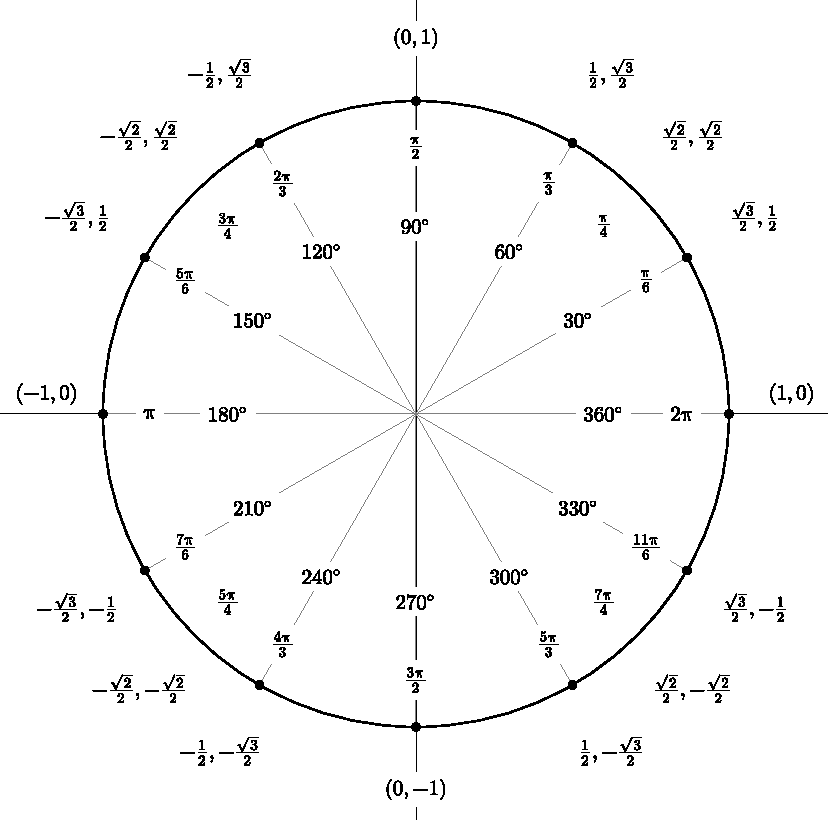
\includegraphics[width=\linewidth]{degrees_circle.pdf}
            
        \definecolor{dg}{RGB}{12, 100, 0}
        \definecolor{db}{RGB}{12, 40, 150}
        \definecolor{dbt}{RGB}{20, 50, 160}
        \definecolor{dr}{RGB}{250, 0, 100}
        \definecolor{dark}{RGB}{100, 100, 100}
        \begin{tikzpicture}
            \begin{axis}%
                [grid=both,
                    minor tick num=4,
                    grid style={line width=.1pt, draw=gray!10},
                    major grid style={line width=.2pt,draw=gray!50},
                    axis lines=middle,
                    enlargelimits={abs=0.4}
                ]
                \addplot[domain=-1.3:1.3,samples=50,smooth,dg] {tan(deg(x))} node[right] {$\tan(x)$};
                \addplot[domain=-6.5:6.5,samples=50,smooth,db] {sin(deg(x))};
                \addplot[domain=-2*pi:2*pi,samples=50,smooth,dr] {cos(deg(x))};
                \node[dbt, above] at (axis cs:-4.6,1) {$\sin(x)$};
                \node[dr, above] at (axis cs:-3,-1.75) {$\cos(x)$};
                \draw[-, line width=0.2mm, dark] (pi,0) -- (pi,0.25) node[above] {$\pi$};
                \draw[-, line width=0.2mm, dark] (-pi,0) -- (-pi,0.25) node[above] {$-\pi$};
                \draw[-, line width=0.2mm, dark] (2*pi,0) -- (2*pi,0.25) node[above] {$2\pi$};    
                \draw[-, line width=0.2mm, dark] (-2*pi,0) -- (-2*pi,0.25) node[above] {$-2\pi$};
                \draw[-, line width=0.1mm, dark] (pi/2,0) -- (pi/2,0.25) node[above] {$\frac{\pi}{2}$};
                \draw[-, line width=0.1mm, dark] (-pi/2,0) -- (-pi/2,0.25) node[above] {$-\frac{\pi}{2}$};
            \end{axis}
        \end{tikzpicture}
        
    \end{center}
    
    \vspace{4cm}
    
    \section{Tabellen}
    \renewcommand{\arraystretch}{1.5}
    
      \subsection{Taylorpolynome}
    \begin{center}
		\begin{tabularx}{\linewidth}{ccX}
			\toprule
			Funktion & $x_0$ & Taylorpolynom \\
  			\hline
			$\sin(x)$ & $0$ & $x - \frac{x^3}{6}+\frac{x^5}{120}-\frac{x^7}{5040}+\frac{x^9}{362880} \ldots$ \\
			$\cos(x)$ & $0$ & $1- \frac{x^2}{2}+\frac{x^4}{24}-\frac{x^6}{720}+\frac{x^8}{40320} \ldots$ \\
			$\tan(x)$ & $0$ & $x+\frac{x^3}{3}+\frac{2 x^5}{15}+\frac{17 x^7}{315}+\frac{62 x^9}{2835} \ldots$ \\
			$\arccos(x)^{(1)}$ & $0$ & $\frac{\pi}{2} - x - \frac{x^3}{6} - \frac{3x^5}{40} - \frac{5x^7}{112} - \frac{35x^9}{1152} - \ldots $ \\
			$\arcsin(x)^{(1)}$ & $0$ & $x + \frac{x^3}{6} + \frac{3x^5}{40} + \frac{5x^7}{112} + \frac{35x^9}{1152} + \ldots$ \\
			$\arctan(x)^{(1)}$ & $0$ & $x-\frac{x^3}{3}+\frac{x^5}{5}-\frac{x^7}{7}+\frac{x^9}{9} \ldots$ \\
			$e^{x}$ & $0$ & $1 + x + \frac{x^2}{2} + \frac{x^3}{6} + \frac{x^4}{24} \ldots$ \\
			$\ln(x)^{(2)}$ & $1$ & $(x\!-\!1) - \frac{(x\!-\!1)^2}{2} + \frac{(x\!-\!1)^3}{3} - \frac{(x\!-\!1)^4}{4}\ldots$ \\
			$\ln(1+x)$ & $0$ & $x- \frac{x^2}{2}+\frac{x^3}{3}-\frac{x^4}{4}+\frac{x^5}{5} \ldots$ \\
			$\sqrt{1+x}$ & $0$ & $1 + \frac{x}{2}-\frac{x^2}{8}+\frac{x^3}{16}-\frac{5x^4}{128} \ldots$ \\
			$\frac{ax}{(b-x)^2}$ & $0$ & $\frac{ax}{b^2}+\frac{2ax^2}{b^3}+\frac{3ax^3}{b^4}+\frac{4ax^4}{b^5}+\frac{5ax^5}{b^6} \ldots$ \\
			\bottomrule
		\end{tabularx}
		Einschränkungen: \hspace{1em} $(1)$:\ $|x|<1$, \hspace{1em}$(2)$:\ $0<x\leq 2$
	\end{center}


    \subsection{Grenzwerte}
    \begin{center}
        \begin{tabularx}{\linewidth}{XX}
            \toprule
            $\limxi \frac{1}{x} = 0$                                   & $\limxi 1 + \frac{1}{x} = 1$             \\
            $\limxi e^x = \infty$                                      & $\limxn e^x = 0$                         \\
            $\limxi e^{-x} = 0$                                        & $\limxn e^{-x} = \infty$                 \\
            $\limxi \frac{e^x}{x^m} = \infty$                          & $\limxn xe^x = 0$                        \\
            $\limxi \ln(x) = \infty$                                   & $\limxo \ln(x) = -\infty$                \\
            $\limxi (1+x)^{\frac{1}{x}} = 1$                           & $\limxo (1+x)^{\frac{1}{x}} = e$         \\
            $\lim_{x\to\pm\infty} (1 + \frac{1}{x})^x = e$             & $\limxi (1-\frac{1}{x})^x = \frac{1}{e}$ \\
            $\limxo \frac{a^x -1}{x} = \ln(a), \newline \forall a > 0$ &                                          
            $\limxi x^a q^x = 0, \newline \forall 0 \le q < 1$ \\
            $\lim_{x\to 1} \frac{\ln(x)}{x-1} = 1$        & $\limxi \frac{\log(x)}{x^a} = 0$   \\
            $\limxi \sqrt[x]{x} = 1$                      & $\limxi \frac{2x}{2^x} = 0$        \\
            \multicolumn{2}{c}{$\lim_{x\to \infty} \left(\sqrt{ax^2+bx+c}-\sqrt{a}\cdot x \right) = \frac{b}{2\sqrt{a}}$} \\
            \bottomrule
        \end{tabularx}
    \end{center}
    
    
    \subsection{Ableitungen}
    \begin{center}
        % the c>{\centering\arraybackslash}X is a workaround to have a column fill up all space and still be centered
        \begin{tabularx}{\linewidth}{c>{\centering\arraybackslash}Xc}
            \toprule
            $\mathbf{F(x)}$                        & $\mathbf{f(x)}$          & $\mathbf{f'(x)}$               \\
            \midrule
            $\frac{x^{-a+1}}{-a+1}$                & $\frac{1}{x^a}$          & $\frac{-a}{x^{a+1}}$            \\
            $\frac{x^{a+1}}{a+1}$                  & $x^a \ (a \ne -1)$       & $a \cdot x^{a-1}$              \\
            $\frac{1}{k \ln(a)}a^{kx}$             & $a^{kx}$                 & $ka^{kx} \ln(a)$               \\
            $\ln |x|$                              & $\frac{1}{x}$            & $-\frac{1}{x^2}$               \\
            $\frac{2}{3}x^{3/2}$                   & $\sqrt{x}$               & $\frac{1}{2\sqrt{x}}$          \\
            $\frac{n}{n+1}x^{\frac{1}{n}+1}$       & $\sqrt[n]{x}$            & $\frac{1}{n}x^{\frac{1}{n}-1}$ \\
            $-\cos(x)$                             & $\sin(x)$                & $\cos(x)$                      \\
            $\sin(x)$                              & $\cos(x)$                & $-\sin(x)$                     \\
            $\frac{1}{2}(x-\frac{1}{2}\sin(2x))$   & $\sin^2(x)$              & $2 \sin(x)\cos(x)$             \\
            $\frac{1}{2}(x + \frac{1}{2}\sin(2x))$ & $\cos^2(x)$              & $-2\sin(x)\cos(x)$             \\
            \multirow{2}*{$-\ln|\cos(x)|$}         & \multirow{2}*{$\tan(x)$} & $\frac{1}{\cos^2(x)}$          \\
                                                    &                          & $1 + \tan^2(x)$                \\
            $\cosh(x)$                             & $\sinh(x)$               & $\cosh(x)$                     \\
            $\log(\cosh(x))$                       & $\tanh(x)$               & $\frac{1}{\cosh^2(x)}$         \\
            $\ln | \sin(x)|$                       & $\cot(x)$                & $-\frac{1}{\sin^2(x)}$         \\
            $\frac{1}{c} \cdot e^{cx}$             & $e^{cx}$                 & $c \cdot e^{cx}$               \\
            $x(\ln |x| - 1)$                       & $\ln |x|$                & $\frac{1}{x}$                  \\
            $\frac{1}{2}(\ln(x))^2$                & $\frac{\ln(x)}{x}$       & $\frac{1 - \ln(x)}{x^2}$       \\
            $\frac{x}{\ln(a)} (\ln|x| -1)$         & $\log_a |x|$             & $\frac{1}{\ln(a)x}$            \\
            \bottomrule
        \end{tabularx}
    \end{center}
    \subsection{Weitere Ableitungen}
    \begin{center}
        \begin{tabularx}{\linewidth}{>{\centering\arraybackslash}X>{\centering\arraybackslash}X}
            \toprule
            $\mathbf{F(x)}$                                     & $\mathbf{f(x)}$                          \\
            \midrule
            $\frac{1}{a\cdot (n+1)}(ax+b)^{n+1}$                & $(ax+b)^n$                               \\
                
            $\arcsin(x)$                                        & $\frac{1}{\sqrt{1 - x^2}}$               \\
            $\arccos(x)$                                        & $\frac{-1}{\sqrt{1 - x^2}}$              \\
            $\arctan(x)$                                        & $\frac{1}{1 + x^2}$                      \\ 
            $\text{arcsinh}(x)$                                 & $\frac{1}{\sqrt{1 + x^2}}$               \\
            $\text{arccosh}(x) $                                & $\frac{1}{\sqrt{x^2 - 1}}$               \\
            $\text{arctanh}(x) $                                & $\frac{1}{1 - x^2}$                      \\ 
            $x^x \ (x > 0)$                                     & $x^x \cdot (1 + \ln x)$                  \\
            $\log_a|x|$                                         & $\frac{1}{x \ln a}=\log_a(e)\frac{1}{x}$ \\
            $\frac{(ax+b)^{n+2}}{a^2(n+1)(n+2)}$                & $\frac{(ax+b)^{n+1}}{a\cdot (n+1)}$      \\
            $\sqrt{1-x^2}+x\cdot \text{arcsin}(x)$              & $\arcsin(x)$                             \\
            $x\cdot \arccos(x)-\sqrt{1-x^2}$                    & $\arccos(x)$                             \\
            $x\cdot \arctan(x)-\frac{1}{2} \log(x^2+1)$         & $\arctan(x)$                             \\ 
            $x\cdot \text{arcsinh}(x)-\sqrt{x^2+1}$             & $\text{arcsinh}(x)$                      \\
            $x\cdot \text{arccosh}(x)-\sqrt{x^2-1}\sqrt{x^2+1}$ & $\text{arccosh}(x)$                      \\
            $\frac{1}{2} \log(1-x^2)+x\cdot \text{arctanh}(x)$  & $\text{arctanh}(x)$                      \\ 
            $\frac{\alpha}{\gamma}\log|\gamma x+\beta|$         & $\frac{\alpha}{\gamma x+\beta}$          \\ 
            \bottomrule
        \end{tabularx}
    \end{center}
    
    \subsection{Definite Integrale}
    \begin{center}
	    $\int_0^{2\pi}\sin(x)=\int_0^{2\pi}\cos(x)=0$, \\$\int_0^{2\pi}\sin^2(x)=\int_0^{2\pi}\cos^2(x)=\pi$    	
    \end{center}

    \subsection{Integrale}
    
    \begin{center}
        \begin{tabularx}{\linewidth}{>{\centering\arraybackslash}X>{\centering\arraybackslash}X}
            \toprule
            $\mathbf{f(x)}$                      & $\mathbf{F(x)}$                                                  \\
            \midrule
            $\int f'(x) f(x) \dx$                & $\frac{1}{2}(f(x))^2$                                            \\
            $\int \frac{f'(x)}{f(x)} \dx$        & $\ln|f(x)|$                                                      \\
            $\int_{-\infty}^\infty e^{-x^2} \dx$ & $\sqrt{\pi}$                                                     \\
            $\int (ax+b)^n \dx$                  & $\frac{1}{a(n+1)}(ax+b)^{n+1}$                                   \\
            $\int x(ax+b)^n \dx$                 & $\frac{(ax+b)^{n+2}}{(n+2)a^2} - \frac{b(ax+b)^{n+1}}{(n+1)a^2}$ \\
            $\int (ax^p+b)^n x^{p-1} \dx$        & $\frac{(ax^p+b)^{n+1}}{ap(n+1)}$                                 \\
            $\int (ax^p + b)^{-1} x^{p-1} \dx$   & $\frac{1}{ap} \ln |ax^p + b|$                                    \\
            $\int \frac{ax+b}{cx+d} \dx$         & $\frac{ax}{c} - \frac{ad-bc}{c^2} \ln |cx +d|$                   \\
            $\int \frac{1}{x^2+a^2} \dx$         & $\frac{1}{a} \arctan \frac{x}{a}$                                \\
            $\int \frac{1}{x^2 - a^2} \dx$       & $\frac{1}{2a} \ln\left| \frac{x-a}{x+a} \right|$                 \\
            $\int \sqrt{a^2+x^2} \dx $           & $\frac{x}{2}f(x) + \frac{a^2}{2}\ln(x+f(x))$                     \\
            \bottomrule
        \end{tabularx}

	
   	\definecolor{grey}{RGB}{100, 100, 100}
   	
    \newcommand{\specialcell}[2][c]{\begin{tabular}[#1]{@{}c@{}}#2\end{tabular}}
    \renewcommand{\arraystretch}{1}
    \vspace{20pt}
    \begin{tabular}{|c|c|c|}
    	\hline \multicolumn{3}{|c|}{ \textbf{Koordinatentransformationen in $\mathbb{R}^2$} } \\
		\hline Definition & \specialcell{Max. Definitions-\\bereich} & Volumenelement \\
		\hline \multicolumn{3}{|c|}{ Polarkoordinaten } \\
		\hline
		$x=r \cos \theta$ & $0 \leq r<\infty$ & $d x d y=r \textcolor{grey}{\ d r d \theta}$ \\
		$y=r \sin \theta$ & $0 \leq \theta<2 \pi$ & \\
		\hline \multicolumn{3}{|c|}{ Elliptische Koordinaten } \\
		\hline
		$x=r a \cos \theta$ & $0 \leq r<\infty$ & $d x d y=$ \\
		$y=r b \sin \theta$ & $0 \leq \theta<2 \pi$ & $a b r \textcolor{grey}{\ d r d \theta}$\\
		\hline \multicolumn{3}{|c|}{ \textbf{Koordinatentransformationen in $\mathbb{R}^3$} } \\
		\hline \multicolumn{3}{|c|}{ Zylinderkoordinaten } \\
		\hline 
		$x=r \cos \theta$ & $0 \leq r<\infty$ & $d x d y d z=$ \\
		$y=r \sin \theta$ & $0 \leq \theta<2 \pi$ & $r \textcolor{grey}{\ d r d \theta d z}$\\
		$z=z$ & $-\infty<z<\infty$ & \\
		\hline \multicolumn{3}{|c|}{ Kugelkoordinaten } \\
		\hline
		$x=r \sin \theta \cos \varphi$ & $0 \leq r<\infty$ & $d x dx y d z=$ \\
		$y=r \sin \theta \sin \varphi$ & $0 \leq \theta \leq \pi$ & $r^2\sin \theta \textcolor{grey}{\ d r d \theta d \varphi}$\\
		$z=r \cos \theta$ & $0 \leq \varphi<2 \pi$ & \\
	\hline
	\end{tabular}
	
	
    \end{center}
    
    	

	    
    	
\end{document}

